% Twelve talk slides and two backup slides. Reuses the thesis evidence and figures.
\documentclass[11pt]{article}
\usepackage[paperwidth=256mm,paperheight=144mm,left=14mm,right=14mm,top=10mm,bottom=10mm]{geometry}
\usepackage{amsmath,booktabs,array,graphicx,xcolor}
\usepackage[hidelinks]{hyperref}
\usepackage{enumitem}
\definecolor{accent}{HTML}{006C80}
\definecolor{ink}{HTML}{182D3D}
\definecolor{muted}{HTML}{536674}
\definecolor{wash}{HTML}{EAF4F5}
\pagestyle{empty}
\setlength{\parindent}{0pt}
\setlength{\parskip}{5pt}
\setlist[itemize]{leftmargin=1.2em,itemsep=5pt,topsep=3pt}
\newcommand{\SiftRecall}{98.99}
\newcommand{\SiftRecallLow}{98.77}
\newcommand{\SiftRecallHigh}{99.22}
\newcommand{\SequentialCycles}{30894}
\newcommand{\RandomCycles}{28968}
\newcommand{\SequentialHit}{96.78}
\newcommand{\RandomHit}{76.85}
\newcommand{\MeanCoverage}{97.7}
\newcommand{\MeanIndexSeconds}{36.89}
\newcommand{\MeanTrainingSeconds}{0.13}
\newcommand{\MeanModelSeconds}{11.17}
\newcommand{\UpperFraction}{9.07}
\newcommand{\QADeltaFloat}{-0.31}
\newcommand{\QALowFloat}{-0.37}
\newcommand{\QAHighFloat}{-0.26}
\newcommand{\QADeltaCompact}{+0.17}
\newcommand{\QALowCompact}{+0.11}
\newcommand{\QAHighCompact}{+0.24}

\newcommand{\GraphRefCompact}{+0.119}
\newcommand{\GraphOneCompact}{-0.191}
\newcommand{\GraphTwoCompact}{-0.705}
\newcommand{\GraphShuffleCompact}{+0.040}
\newcommand{\GraphRecallMin}{98.55}
\newcommand{\GraphRecallMax}{99.35}
\newcommand{\SequentialBanks}{2.97}
\newcommand{\RandomBanks}{14.81}
\newcommand{\SavedCyclesPerQuery}{97.3}
\newcommand{\MixedDeltaCycles}{2,848}
\newcommand{\MixedSavedCommands}{25,125}
\newcommand{\MixedExtraNoCommand}{27,973}
\newcommand{\MixedSavedACT}{12,516}
\newcommand{\BfsOfferedBanks}{14.62}
\newcommand{\QAOfferedBanks}{13.88}
\newcommand{\MappingMiB}{1.53}

\newcommand{\MeanPhasesPerQuery}{146.5}
\newcommand{\MeanVectorsPerPhase}{13.80}
\newcommand{\RRCmdExtraFloat}{277,894}
\newcommand{\RRNoCmdDeltaFloat}{1,429,356}
\newcommand{\RRStreamDeltaFloat}{1,151,462}
\newcommand{\RRBanksBeforeFloat}{4.75}
\newcommand{\RRHitBeforeFloat}{93.41}
\newcommand{\RRBanksAfterFloat}{15.07}
\newcommand{\RRHitAfterFloat}{89.23}
\newcommand{\QABoundedFloat}{-0.21 [-0.27, -0.15]}
\newcommand{\PorderBoundedFloat}{-0.38 [-0.47, -0.28]}
\newcommand{\GorderBoundedFloat}{-0.20 [-0.24, -0.16]}
\newcommand{\RCMBoundedFloat}{-0.16 [-0.21, -0.11]}
\newcommand{\SortedBFSFloat}{+0.19 [+0.13, +0.24]}
\newcommand{\SortedBFSMeanFloat}{+0.19}
\newcommand{\SortedBFSSavedFloat}{-75}
\newcommand{\RoundRobinBFSFloat}{-14.58 [-14.64, -14.51]}
\newcommand{\RoundRobinBFSMeanFloat}{-14.58}
\newcommand{\RoundRobinBFSSavedFloat}{5,802}
\newcommand{\RRFasterQueriesFloat}{100.0}
\newcommand{\RRPtailRangeFloat}{-15.24 to -13.61}
\newcommand{\RRCmdExtraCompact}{49,970}
\newcommand{\RRNoCmdDeltaCompact}{53,465}
\newcommand{\RRStreamDeltaCompact}{103,435}
\newcommand{\RRBanksBeforeCompact}{14.10}
\newcommand{\RRHitBeforeCompact}{76.49}
\newcommand{\RRBanksAfterCompact}{18.50}
\newcommand{\RRHitAfterCompact}{73.45}
\newcommand{\QABoundedCompact}{+0.10 [+0.01, +0.18]}
\newcommand{\PorderBoundedCompact}{-1.19 [-1.33, -1.04]}
\newcommand{\GorderBoundedCompact}{-1.33 [-1.42, -1.25]}
\newcommand{\RCMBoundedCompact}{-0.47 [-0.55, -0.38]}
\newcommand{\SortedBFSCompact}{+0.17 [+0.12, +0.21]}
\newcommand{\SortedBFSMeanCompact}{+0.17}
\newcommand{\SortedBFSSavedCompact}{-26}
\newcommand{\RoundRobinBFSCompact}{+3.43 [+3.31, +3.55]}
\newcommand{\RoundRobinBFSMeanCompact}{+3.43}
\newcommand{\RoundRobinBFSSavedCompact}{-541}
\newcommand{\RRFasterQueriesCompact}{6.0--15.0}
\newcommand{\RRPtailRangeCompact}{+3.22 to +6.36}

\newcommand{\SchedRaisedLimitEqual}{60}
\newcommand{\SchedDefaultPeak}{50}
\newcommand{\SchedDefaultSortFloat}{+0.19}
\newcommand{\SchedDefaultRRFloat}{-14.58}
\newcommand{\SchedDefaultSortCompact}{+0.17}
\newcommand{\SchedDefaultRRCompact}{+3.43}
\newcommand{\SchedInflightSixteenSortFloat}{+0.28}
\newcommand{\SchedInflightSixteenRRFloat}{-33.08}
\newcommand{\SchedInflightSixteenSortCompact}{+0.71}
\newcommand{\SchedInflightSixteenRRCompact}{-10.61}
\newcommand{\SchedInflightThirtyTwoSortFloat}{+0.26}
\newcommand{\SchedInflightThirtyTwoRRFloat}{-21.86}
\newcommand{\SchedInflightThirtyTwoSortCompact}{+0.29}
\newcommand{\SchedInflightThirtyTwoRRCompact}{+1.62}
\newcommand{\SchedInflightOneTwentyEightSortFloat}{+0.19}
\newcommand{\SchedInflightOneTwentyEightRRFloat}{-14.58}
\newcommand{\SchedInflightOneTwentyEightSortCompact}{+0.17}
\newcommand{\SchedInflightOneTwentyEightRRCompact}{+3.43}
\newcommand{\SchedBatchTwoSortFloat}{-0.07}
\newcommand{\SchedBatchTwoRRFloat}{-7.77}
\newcommand{\SchedBatchTwoSortCompact}{-0.08}
\newcommand{\SchedBatchTwoRRCompact}{-1.48}
\newcommand{\SchedBatchEightSortFloat}{+0.13}
\newcommand{\SchedBatchEightRRFloat}{-15.55}
\newcommand{\SchedBatchEightSortCompact}{+0.13}
\newcommand{\SchedBatchEightRRCompact}{-2.48}
\newcommand{\SchedAlternateMappingSortFloat}{+3.52}
\newcommand{\SchedAlternateMappingRRFloat}{+112.71}
\newcommand{\SchedAlternateMappingSortCompact}{-0.34}
\newcommand{\SchedAlternateMappingRRCompact}{+42.59}
\newcommand{\RRvsPublishedFloat}{-14.25}
\newcommand{\RRvsPublishedLowFloat}{-14.36}
\newcommand{\RRvsPublishedHighFloat}{-14.14}
\newcommand{\RRvsPublishedCompact}{+4.82}
\newcommand{\RRvsPublishedLowCompact}{+4.69}
\newcommand{\RRvsPublishedHighCompact}{+4.96}

\newcommand{\ProfileMaxMeanRegret}{0.000}
\newcommand{\ProfileMaxSplitRegret}{0.000}
\newcommand{\ProfileWorstOriginal}{+0.000}
\newcommand{\ProfileOracleMatches}{140}
\newcommand{\ProfileOriginalRegressions}{0}
\newcommand{\ProfileOriginalChoices}{40}
\newcommand{\ProfileSortedChoices}{10}
\newcommand{\ProfileRRChoices}{90}
\newcommand{\ProfileDefaultFloat}{-14.58}
\newcommand{\ProfileInflightSixteenFloat}{-33.08}
\newcommand{\ProfileInflightThirtyTwoFloat}{-21.86}
\newcommand{\ProfileInflightOneTwentyEightFloat}{-14.58}
\newcommand{\ProfileBatchTwoFloat}{-7.77}
\newcommand{\ProfileBatchEightFloat}{-15.55}
\newcommand{\ProfileAlternateMappingFloat}{+0.00}
\newcommand{\ProfileVsRcmFloat}{-14.44 [-14.53, -14.35]}
\newcommand{\ProfileVsGorderFloat}{-14.40 [-14.50, -14.31]}
\newcommand{\ProfileVsPorderFloat}{-14.25 [-14.36, -14.14]}
\newcommand{\ProfileDefaultCompact}{+0.00}
\newcommand{\ProfileInflightSixteenCompact}{-10.61}
\newcommand{\ProfileInflightThirtyTwoCompact}{+0.00}
\newcommand{\ProfileInflightOneTwentyEightCompact}{+0.00}
\newcommand{\ProfileBatchTwoCompact}{-1.48}
\newcommand{\ProfileBatchEightCompact}{-2.48}
\newcommand{\ProfileAlternateMappingCompact}{-0.34}
\newcommand{\ProfileVsRcmCompact}{+0.47 [+0.38, +0.56]}
\newcommand{\ProfileVsGorderCompact}{+1.35 [+1.26, +1.44]}
\newcommand{\ProfileVsPorderCompact}{+1.20 [+1.05, +1.35]}

\newenvironment{slide}[2]{%
  \clearpage\color{ink}\fontsize{14}{18}\selectfont
  {\fontsize{10}{12}\selectfont\color{accent}\MakeUppercase{#1}\par}
  {\fontsize{25}{29}\selectfont\bfseries #2\par}\vspace{4pt}
}{%
  \vfill{\color{accent}\hrule}\vspace{4pt}
  {\fontsize{9}{11}\selectfont\color{muted}Artashes Atanesyan\hfill DRAM locality in graph-based ANN\hfill\thepage\par}
}
\newcommand{\takeaway}[1]{\par\vspace{3pt}\colorbox{wash}{\parbox{\dimexpr\linewidth-2\fboxsep\relax}{\strut\textbf{#1}\strut}}\par}
\newcommand{\evidence}[2]{\vfill{\fontsize{9}{11}\selectfont\color{muted}Evidence: \href{https://github.com/senqx/Thesis-PIM-ANN/blob/main/#1}{#2}. Links open the maintained artifact; pin a Git revision for reproduction.\par}}
\begin{document}
\hypersetup{pdftitle={DRAM locality in graph-based ANN: thesis defence},pdfauthor={Artashes Atanesyan}}

\begin{slide}{Master's thesis defence}{When does better locality make memory slower?}
\vspace{6pt}
{\fontsize{20}{25}\selectfont DRAM locality in graph-based\newline approximate nearest neighbour search\par}
\vspace{10pt}
Artashes Atanesyan\hfill 10 November 2026

\textbf{Question:} if graph search needs the same data, can changing its\newline placement and the order of available reads finish memory service sooner?

\takeaway{Row reuse saves operations. Bank parallelism can hide waiting.}
We follow this tension from controlled traces to HNSW graph search,\newline then to a proposed processing-in-memory (PIM) interface.
\evidence{doc/pim_ann_thesis.pdf}{Full thesis; simulated DRAM service, not measured application/PIM speedup}
\end{slide}

\begin{slide}{1 / Research contribution}{Three questions, one controlled comparison}
\begin{minipage}[t]{0.49\linewidth}
\textbf{RQ1 --- Access order}\par
How do order, runs and presorting interact with request concurrency?
\par\textbf{RQ2 --- Graph-search choices}\par
Which placements and available-read schedules help? Can training select one?
\par\textbf{RQ3 --- Robustness}\par
Which conclusions survive the selected footprint, boundary, controller and graph changes?
\end{minipage}\hfill
\begin{minipage}[t]{0.47\linewidth}
\textbf{Established prior work}\par
Gorder: general graph ordering.\newline
Porder: profile-guided ANN placement.\newline
PIM-ANN systems: complete system designs with different execution costs.
\par\textbf{This thesis adds}\par
Fixed-search comparisons in a specified HBM2 model, command evidence for reversals, and bounded scheduling with explicit costs and limits.
\end{minipage}
\evidence{doc/RESEARCH_POSITION.md}{Research position and cited prior work; selected references on slide 14}
\end{slide}

\begin{slide}{2 / Experimental contract}{Change addresses and order; preserve search work}
\vspace{5pt}
\begin{center}\fontsize{13}{17}\selectfont
\colorbox{wash}{\parbox[c][22mm][c]{0.20\linewidth}{\centering\textbf{Search}\par Discover\newline candidate IDs}}
$\rightarrow$
\colorbox{wash}{\parbox[c][22mm][c]{0.20\linewidth}{\centering\textbf{Placement}\par Map IDs to\newline vector addresses}}
$\rightarrow$
\colorbox{wash}{\parbox[c][22mm][c]{0.20\linewidth}{\centering\textbf{Request order}\par Offer native\newline memory reads}}
$\rightarrow$
\colorbox{wash}{\parbox[c][22mm][c]{0.20\linewidth}{\centering\textbf{Controller}\par Measure completed\newline service cycles}}
\end{center}\vspace{10pt}
\begin{minipage}[t]{0.49\linewidth}
\textbf{Workload}\par
HNSW: graph-based approximate nearest neighbours; SIFT100k, 128 dimensions.\newline
Ten paired splits; 200 held-out queries each. Mean Recall@10: \SiftRecall\%.
\end{minipage}\hfill
\begin{minipage}[t]{0.47\linewidth}
\textbf{Memory model}\par
Pinned Ramulator 2.1, one HBM2 channel.\newline
512-byte float32 vector: 16 native reads.\newline
Hypothetical 128-byte vector: 4 reads,\newline with the same float32 traversal and recall.
\end{minipage}
\evidence{doc/REPRODUCIBILITY.md}{Fixed traces, stock-search comparisons, native 32-byte accounting and paired protocol}
\end{slide}

\begin{slide}{3 / What can the controller see?}{Execution boundaries change available parallelism}
\vspace{6pt}
\begin{center}\renewcommand{\arraystretch}{1.9}
\begin{tabular}{ll}
\textbf{Flat replay} & List $\rightarrow$ v1, v2, v3, v4 $\rightarrow$ next list \\
\textbf{Expansion phases} & List \textcolor{accent}{$\;|\;$} v1, v2, v3, v4 \textcolor{accent}{$\;|\;$} next list \\
\textbf{Batches of two} & List \textcolor{accent}{$\;|\;$} v1, v2 \textcolor{accent}{$\;|\;$} v3, v4 \textcolor{accent}{$\;|\;$} next list
\end{tabular}\end{center}
\takeaway{Each divider means: finish every read in this group before offering the next.}
List = neighbour IDs. v1--v4 = vectors needed by those candidates.\par
\textbf{Flat replay} offers known future demand early. \textbf{Bounded replay} waits\newline for memory groups, but executes no distance computation or control logic.
\evidence{doc/followup_methods.tex}{Replay models; list = neighbour IDs, v1--v4 = candidate vectors; rows stay warm across drains}
\end{slide}

\begin{slide}{4 / Start with placement}{A measurable effect can have little practical value}
\textbf{Query-aware placement versus breadth-first (BFS) placement}\par
Default flat replay, same search work; ten paired split effects.
\vspace{4pt}
\begin{center}\renewcommand{\arraystretch}{1.25}
\begin{tabular}{lrr}\toprule
Vector footprint & Mean cycle change & Paired 95\% interval \\\midrule
512 bytes & \QADeltaFloat\% & [\QALowFloat, \QAHighFloat]\% \\
128 bytes (hypothetical) & \QADeltaCompact\% & [\QALowCompact, \QAHighCompact]\% \\\bottomrule
\end{tabular}\end{center}
\begin{itemize}
\item \textbf{Statistical:} the conditional intervals exclude zero.
\item \textbf{Practical:} only about \SavedCyclesPerQuery{} cycles/query saved at 512 bytes, before layout and integration costs.
\item \textbf{Architectural:} the 128-byte layout has more row hits yet takes longer. Row-hit fraction alone cannot choose a layout.
\end{itemize}
\evidence{doc/generated/real_table.tex}{Generated primary placement table; published Gorder/Porder comparisons retained separately}
\end{slide}

\begin{slide}{5 / Stronger scheduling contrast}{Round-robin helps one footprint and hurts the other}
{\fontsize{12}{15}\selectfont Round-robin interleaves chunks of available vectors; original order offers each vector's chunks together.\par}
\begin{center}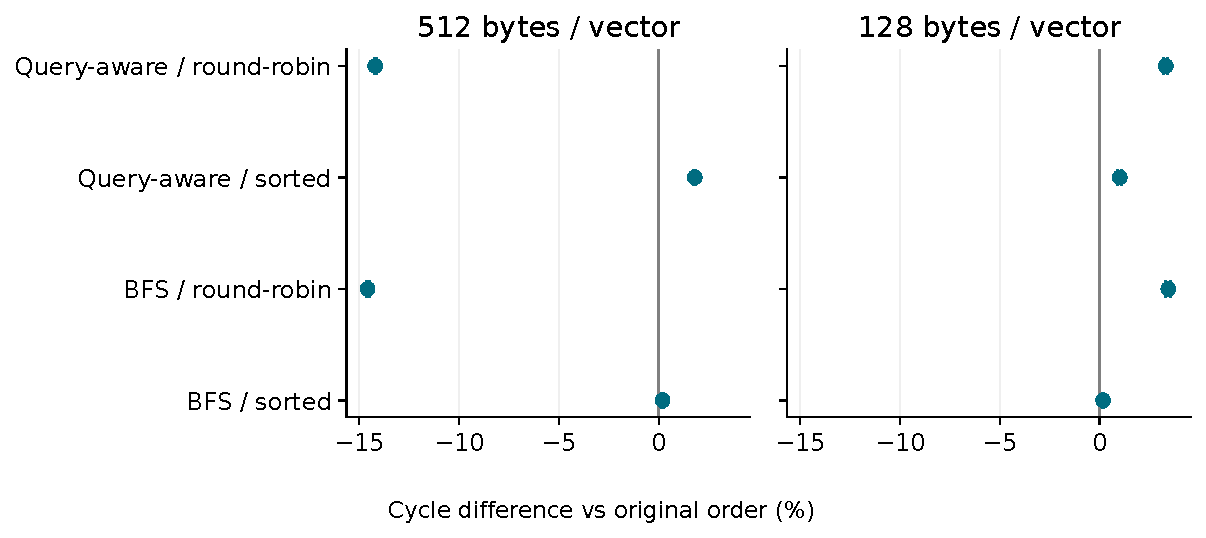
\includegraphics[width=0.94\linewidth,height=62mm,keepaspectratio]{generated/followup_schedules.pdf}\end{center}
\textbf{BFS:} \RoundRobinBFSMeanFloat\% at 512 bytes; \RoundRobinBFSMeanCompact\% at hypothetical 128 bytes.
\evidence{results/followup_summary.csv}{Expansion-bounded schedules, ten paired splits; bars = 95\% intervals; negative = fewer cycles}
\end{slide}

\begin{slide}{6 / Why locality can lose}{More row operations, much less waiting}
Reference split 1: expansion-bounded BFS, 512 bytes, round-robin versus original.
\begin{center}\renewcommand{\arraystretch}{1.18}
\begin{tabular}{lrr}\toprule
Diagnostic & Original & Round-robin \\\midrule
Row-hit fraction & \RRHitBeforeFloat\% & \RRHitAfterFloat\% \\
Offered bank diversity & \RRBanksBeforeFloat & \RRBanksAfterFloat \\\bottomrule
\end{tabular}\end{center}
\begin{center}
{\fontsize{19}{23}\selectfont
$\underbrace{+277{,}894}_{\text{command cycles}}\quad-\quad
\underbrace{1{,}429{,}356}_{\text{no-command cycles}}\quad=\quad
\underbrace{-1{,}151{,}462}_{\text{total cycles}}$}
\end{center}
\takeaway{The additional row work is outweighed by less idle service time.}
{\fontsize{12}{15}\selectfont Bank diversity counts distinct banks in 64-request input windows, not live queue occupancy. No-command cycles include several causes; this is one diagnostic split, not a new statistical replication.\par}
\evidence{doc/generated/followup_mechanism_table.tex}{Generated command accounting; the same mechanism does not guarantee a gain at 128 bytes}
\end{slide}

\begin{slide}{7 / Test the recommendation}{Footprint alone cannot select a schedule}
\begin{center}\renewcommand{\arraystretch}{1.13}\fontsize{13}{16}\selectfont
\begin{tabular}{lrr}\toprule
Round-robin vs. matching original BFS & 512 bytes & 128 bytes* \\\midrule
Default: 64 outstanding & \SchedDefaultRRFloat\% & \SchedDefaultRRCompact\% \\
16 outstanding & \SchedInflightSixteenRRFloat\% & \SchedInflightSixteenRRCompact\% \\
32 outstanding & \SchedInflightThirtyTwoRRFloat\% & \SchedInflightThirtyTwoRRCompact\% \\
128 outstanding & \SchedInflightOneTwentyEightRRFloat\% & \SchedInflightOneTwentyEightRRCompact\% \\
Candidate batches of 2 & \SchedBatchTwoRRFloat\% & \SchedBatchTwoRRCompact\% \\
Candidate batches of 8 & \SchedBatchEightRRFloat\% & \SchedBatchEightRRCompact\% \\
Alternative address mapping & \SchedAlternateMappingRRFloat\% & \SchedAlternateMappingRRCompact\% \\\bottomrule
\end{tabular}\end{center}
\takeaway{The same order can help or hurt as execution constraints change.}
{\fontsize{12}{15}\selectfont Ten paired split means. Only the named setting changes. *Hypothetical footprint.\newline
The 128-outstanding cap is nonbinding: all \SchedRaisedLimitEqual{} records match default cycles.\par}
\evidence{results/scheduling_summary.csv}{Complete sensitivity matrix with paired intervals, sorting, absolute savings and query effects}
\end{slide}

\begin{slide}{8 / A modest engineering proposal}{Profile once, then use a fixed order}
\takeaway{50 training queries $\times$ 3 orders $\longrightarrow$ freeze the choice $\longrightarrow$ 200 held-out queries}
\begin{minipage}[t]{0.48\linewidth}
\textbf{Observed}\par
\ProfileOracleMatches/140 choices match the best of the three fixed held-out orders.\par
$7$ settings $\times$ $2$ footprints $\times$ $10$ splits, on one graph and query pool.\par
Original / sorted / round-robin:\newline
\ProfileOriginalChoices{} / \ProfileSortedChoices{} / \ProfileRRChoices{} choices.
\end{minipage}\hfill
\begin{minipage}[t]{0.48\linewidth}
\textbf{Interpretation}\par
Exploratory: inspected test outcomes motivated the policy. No universal success rate or benefit over a correctly chosen fixed schedule is established.\par
Default 512-byte selected BFS vs. Porder: \mbox{\ProfileVsPorderFloat\%}.\newline
At 128 bytes vs. Gorder: \mbox{\ProfileVsGorderCompact\%}. Individual-query losses remain.
\end{minipage}
\evidence{doc/profiled_fetch_results.tex}{Training-only choice rule, fixed alternatives, published baselines, costs and limitations}
\end{slide}

\begin{slide}{9 / Does the gain pay for itself?}{The implementation has an overhead budget}
\begin{minipage}[t]{0.48\linewidth}
\textbf{Default bounded BFS, 512 bytes}\par
About \RoundRobinBFSSavedFloat{} service cycles saved per query before extra costs.\par
Mean calibration: 5,716,851 cycles.\newline
Calibration / saving $\approx$ 985 queries.\par
If extra work consumes half the saving,\newline the ratio becomes about 1,971 queries.
\end{minipage}\hfill
\begin{minipage}[t]{0.48\linewidth}
\textbf{What can erase it?}\par
Additional dispatch, address mapping, buffering, synchronisation and transfers. Charge incremental costs when comparing schedules on the same engine.\par
The 200 held-out queries save only\newline 1.16 million service cycles, less than\newline 5.72 million spent on calibration.
\end{minipage}
\takeaway{A correct fixed schedule earns the same replay benefit without repeating calibration.}
{\fontsize{12}{15}\selectfont Ratios of retained means under stable, serial additive costs; not measured deployment break-even. Workload lifetime, overlap, drift and real engine costs remain unknown.\par}
\evidence{doc/profiled_fetch_results.tex}{Worked amortisation example; raw selection and cost summaries retained}
\end{slide}

\begin{slide}{10 / Why this matters for PIM}{A concrete interface to evaluate next}
\textbf{Proposed, not implemented:} keep vectors resident and return tagged distances.\par
\vspace{6pt}
\colorbox{wash}{\parbox[t]{0.44\linewidth}{\textbf{Host control}\par
Read neighbour IDs from DRAM.\newline
Maintain queues and visited state.\newline
Resolve candidate vector addresses.}}
\hfill
\colorbox{wash}{\parbox[t]{0.44\linewidth}{\textbf{Near-memory engine}\par
Retain query in local storage.\newline
Gather resident vectors in chosen order.\newline
Compute and tag their distances.}}
\begin{center}\fontsize{13}{17}\selectfont
Host $\xrightarrow{\text{query once; then addresses + tags}}$ engine\\[4pt]
Host $\xleftarrow{\text{distances + tags}}$ engine
\end{center}
{\fontsize{12}{16}\selectfont Requires local arithmetic/storage, tagged fine-grained requests and compatible mapping. Preserve numerical, tie and search-update semantics. Whole-vector or bank-local interfaces may not expose the tested ordering.\par}
\takeaway{DRAM scheduling guides this interface; complete PIM performance remains unmeasured.}
\evidence{doc/execution_sketch.tex}{Residency, transferred data, hardware requirements and unmeasured execution costs}
\end{slide}

\begin{slide}{11 / Answers and scope}{Choose with completed service, then check full cost}
\textbf{RQ1:} locality and concurrency interact. Access order can reverse a\newline ranking; neither row hits nor contiguous runs alone establish lower time.
\par\textbf{RQ2:} named placements and schedules provide conditional alternatives.\newline Profiling selects useful fixed orders in this exploratory matrix.
\par\textbf{RQ3:} several rankings reverse under the tested changes.\newline The evidence does not establish a universal schedule or footprint rule.
\takeaway{Footprint $+$ available work $+$ mapping $+$ boundaries determine the useful memory schedule.}
\textbf{Demonstrated:} reproducible service comparisons and positive/negative results.\newline
\textbf{Still required for PIM speedup:} implemented compute, buffers, transfers,\newline scheduling costs, and end-to-end validation at equal recall and concurrency.
\evidence{doc/VALIDATION.md}{Current PDFs and validation; 2,069 records = 1,289 previous + 360 sensitivity + 420 calibration}
\end{slide}

\begin{slide}{Backup / Defence boundaries}{What the evidence can and cannot answer}
\begin{itemize}
\item \textbf{Why ten splits?} They quantify paired query variation on one graph. Overlapping pools and exploratory comparisons limit inference; they do not establish hardware or dataset generality.
\item \textbf{Why 128 bytes?} A controlled traffic/packing sensitivity with float32 search held fixed. Quantisation accuracy and arithmetic were not evaluated.
\item \textbf{Why HNSW/SIFT100k?} A reproducible graph-search operating point; one real corpus, one main parameter/recall setting. Three additional graph constructions test limited variation.
\item \textbf{What is validated?} Retained accounting, membership, source identities, analysis regeneration and three separate fresh simulations. The simulator has not been validated against physical PIM hardware here.
\end{itemize}
\evidence{doc/READING_GUIDE.md}{Thirteen expanded defence answers; reproduction inventory and historical-baseline distinction}
\end{slide}

\begin{slide}{Backup / Selected references}{Established methods frame the contribution}
{\fontsize{12}{16}\selectfont
\textbf{Graph search.} Malkov and Yashunin, HNSW, IEEE TPAMI 42(4), 2020.\newline
\href{https://doi.org/10.1109/TPAMI.2018.2889473}{doi:10.1109/TPAMI.2018.2889473}
\par\textbf{Placement.} Wei et al., Gorder, SIGMOD 2016, pp. 1813--1828.\newline
\href{https://doi.org/10.1145/2882903.2915220}{doi:10.1145/2882903.2915220}. Coleman et al., graph reordering / Porder, NeurIPS 35, 2022.\newline
\href{https://doi.org/10.52202/068431-2789}{doi:10.52202/068431-2789}
\par\textbf{DRAM model.} Luo et al., Ramulator 2.0, IEEE CAL 23(1), 2024.\newline
\href{https://doi.org/10.1109/LCA.2023.3333759}{doi:10.1109/LCA.2023.3333759}. Experiments pin the later Ramulator 2.1 source.
\par\textbf{PIM systems.} DRIM-ANN and UpANNS, SC 2025; PIMANN, USENIX ATC 2025.\newline
PIMCQG, arXiv:2605.25522v2; public record states SC26 acceptance (checked 10 Nov. 2026).
\par Full citations, publication status and the architectural distinctions are in the thesis bibliography and related-work section.\par}
\evidence{doc/references.tex}{Shared thesis/IEEE bibliography; talk guidance in READING\_GUIDE.md}
\end{slide}
\end{document}
